\documentclass{beamer}
\usetheme{Boadilla}
\usepackage{bibentry}
\usepackage{cmbright}
\usepackage{natbib}
\setbeamertemplate{itemize items}[circle]
\setbeamertemplate{enumerate items}[default]

\def\E{\text{E}}
\def\Var{\text{Var}}
\def\Cov{\text{Cov}}

\title[Euler Equation]{Work in Progress: The Euler Equation Implied Rate Under Heterogeneous Preferences}
\author[Li]{Pearl Li}
\date{February 3, 2016}

\begin{document}

\begin{frame}
\titlepage
\end{frame}


\begin{frame}{Last Time}
\begin{itemize}
\item Literature review
\item Cleaned raw data from FRED
\item Estimated VAR(4) for consumption, inflation, leisure, FFR, ...
\item Computed implied interest rates under CRRA utility
  \begin{itemize}
  \item Implied real rates corresponded well to \cite{collard11}
  \item Implied nominal rates were very bad...
  \end{itemize}
\end{itemize}
\end{frame}

\begin{frame}{Last Time}
\begin{center}
\begin{tabular}{cc}
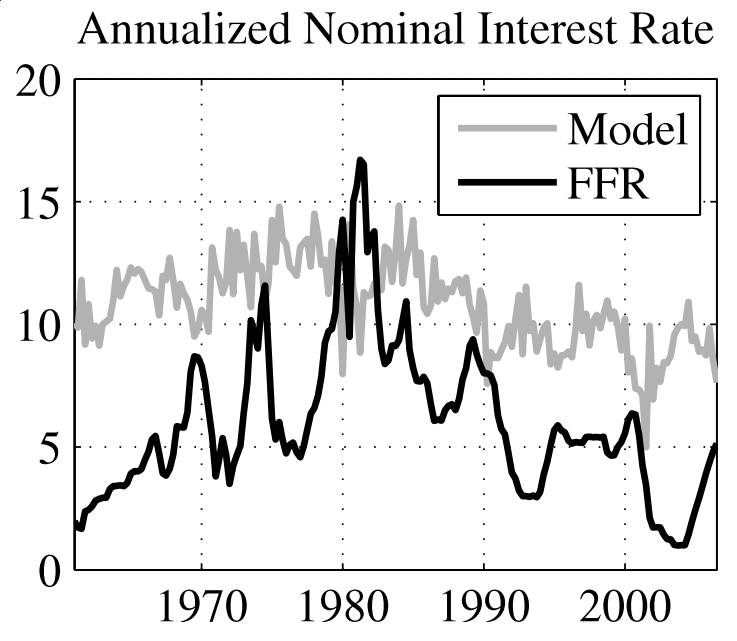
\includegraphics[height=120px]{figs/old/crra-nominal_collard.png} &
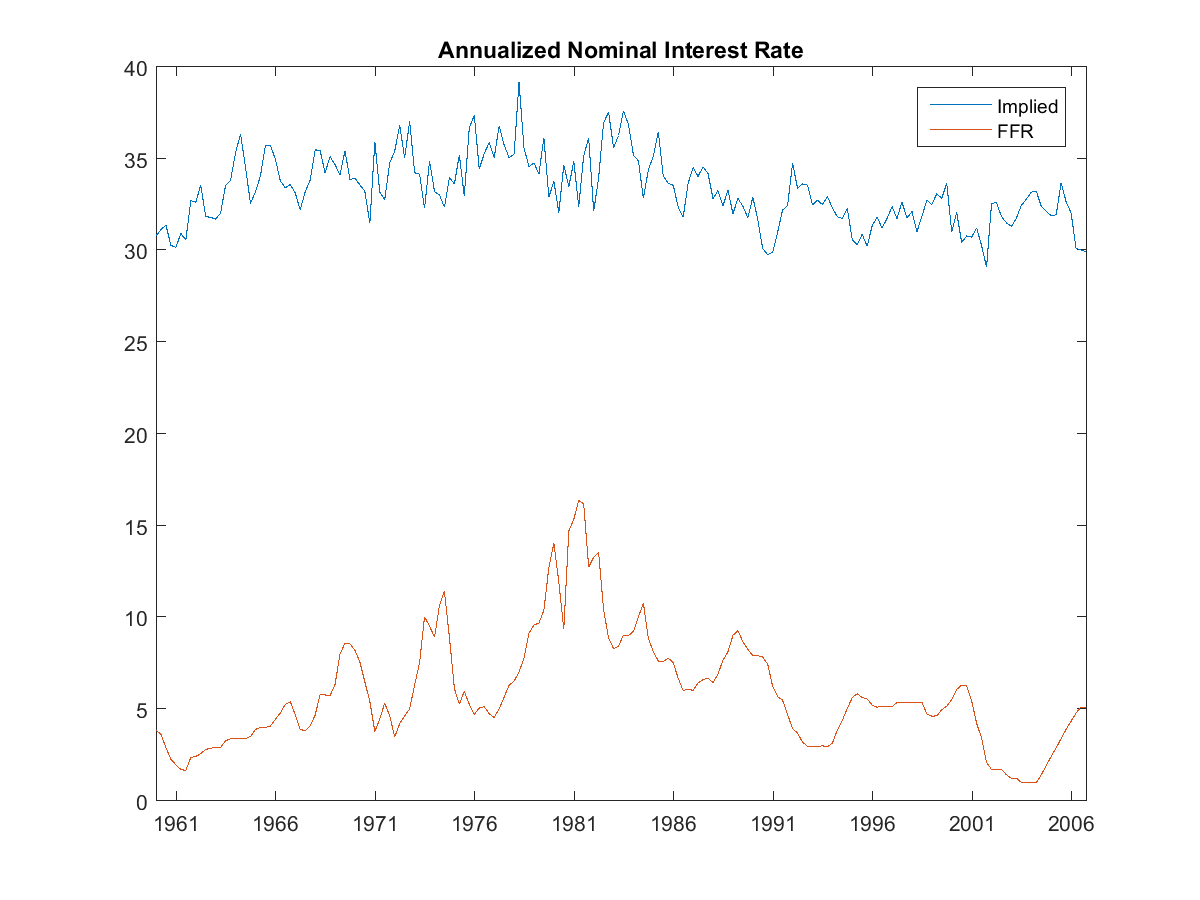
\includegraphics[height=120px]{figs/old/crra-nominal.png} \\
\cite{collard11} & Li (2015)
\end{tabular}
\end{center}
\begin{itemize}
\item It turns out this resulted from a matrix indexing error
\end{itemize}
\end{frame}

\begin{frame}{Generalized Implied Rates}
\begin{itemize}
\item As in \cite{collard11}: $$u(C_t, \ell_t) = \frac{[(C_t/C_{t-1}^\varphi)^\nu \ell_t^{1-\nu}]^{1-\alpha}}{1-\alpha}$$
\item Discount factor $\beta = 0.9926$
\item Coefficient of risk aversion $\alpha = 2$
\item \textbf{Habit persistence parameter $\varphi = 0.8$}
\item \textbf{Weight assigned to consumption $\nu = 0.34$}
\item When $\varphi = 0$ and $\nu = 1$, this reduces to CRRA utility (last time)
\end{itemize}
\end{frame}

\begin{frame}{Generalized Implied Rates}
\begin{itemize}
\item Euler equation (from first-order conditions)
  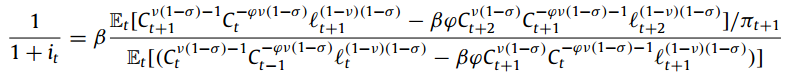
\includegraphics[width=0.9\textwidth]{figs/euler-equation.png}
\item Assuming conditional lognormality, nominal interest rate given by
$$\frac{1}{1+i_t} = \beta \frac{\exp(\chi_{1t}) - \beta \varphi \exp(\chi_{2t})}{\exp(\chi_{3t}) - \beta \varphi \exp(\chi_{4t})}$$
\begin{align*}
\chi_{1t} &= (\nu(1-\alpha)-1) \E_t c_{t+1} - \varphi\nu(1-\alpha)c_t + (1-\nu)(1-\alpha) \E_t \ell_{t+1} \\
  &\qquad - \E_t \pi_{t+1} + \text{constant second-order moments} \\
\chi_{2t} &= \ldots
\end{align*}
\item Real interest rate is same without inflation terms
\end{itemize}
\end{frame}

\begin{frame}{Treatments}
$$u(C_t, \ell_t) = \frac{[(C_t/C_{t-1}^\varphi)^\nu \ell_t^{1-\nu}]^{1-\alpha}}{1-\alpha}$$
\begin{itemize}
\item $\varphi = 0, \nu = 1$: CRRA (SEP)
\item $\varphi = 0.8, \nu = 1$: habit persistence (SEP + HP)
\item $\varphi = 0, \nu = 0.34$: non-separable consumption and leisure (NSEP)
\item $\varphi = 0.8, \nu = 0.34$: non-separable consumption and leisure + habit persistence (NSEP + HP)
\end{itemize}
\end{frame}

\begin{frame}{Results: SEP}
\begin{center}
\begin{tabular}{cc}
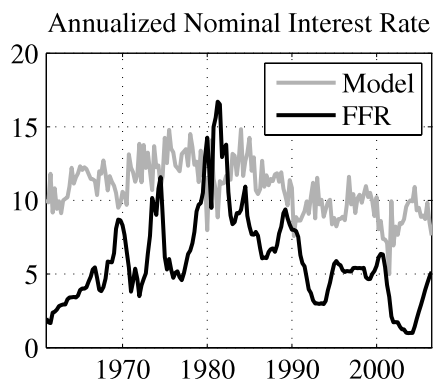
\includegraphics[height=90px]{figs/implied_ffr/nominal_1_collard.png} &
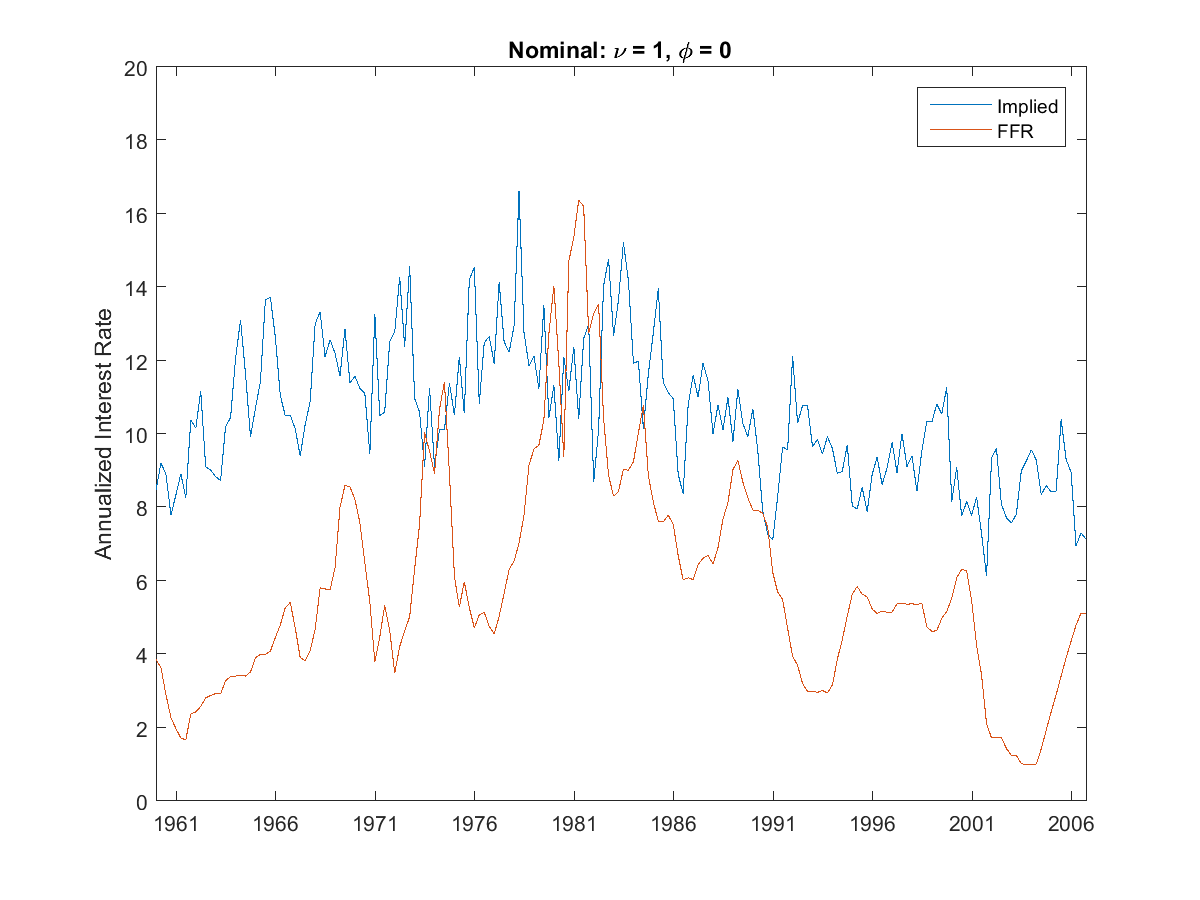
\includegraphics[height=90px]{figs/implied_ffr/nominal_1.png} \\
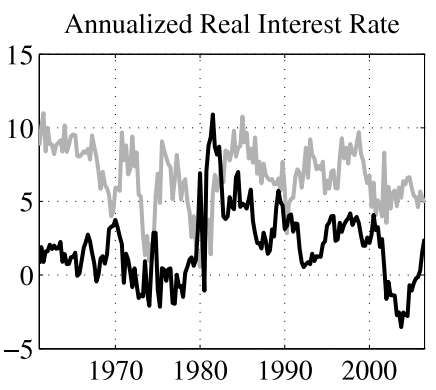
\includegraphics[height=90px]{figs/implied_ffr/real_1_collard.png} &
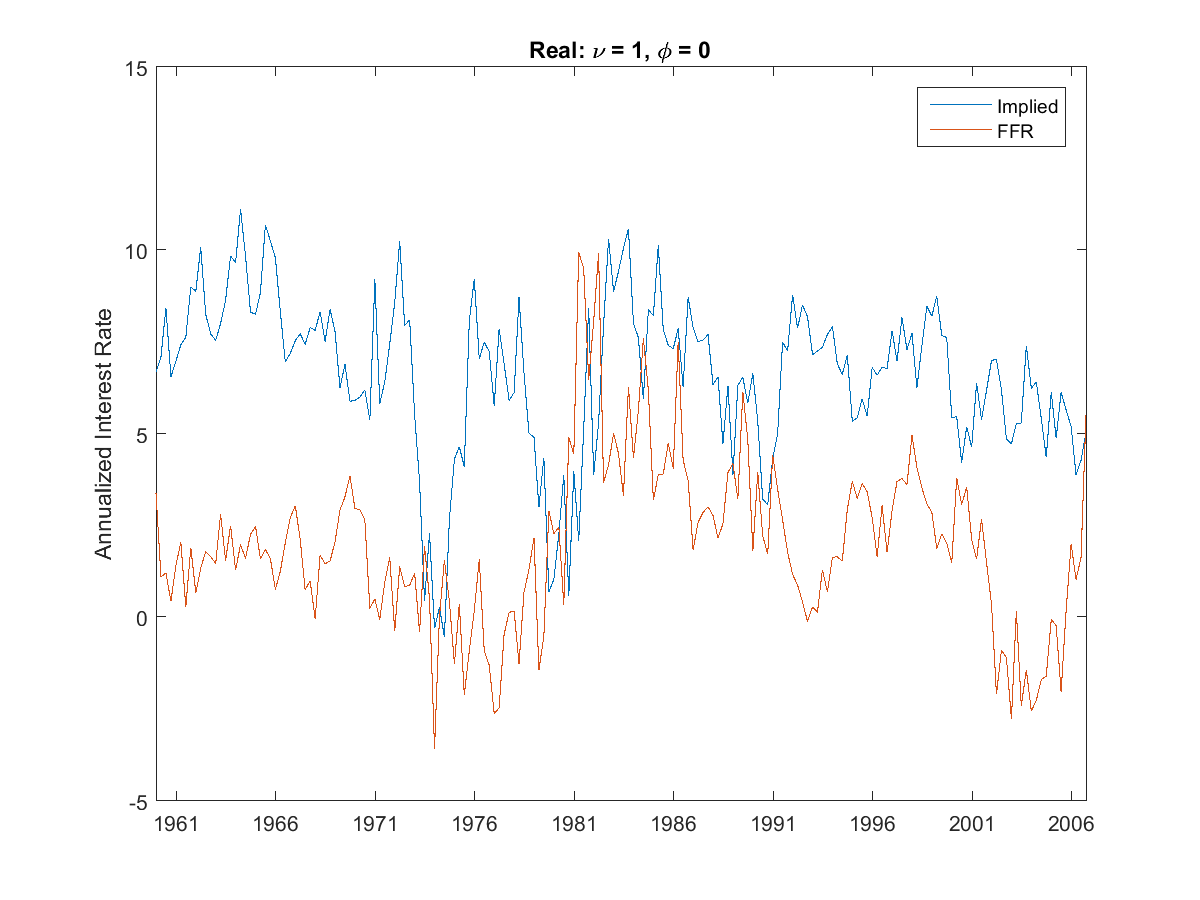
\includegraphics[height=90px]{figs/implied_ffr/real_1.png} \\
\cite{collard11} & Li (2016)
\end{tabular}
\end{center}
\end{frame}

\begin{frame}{Results: SEP + HP}
\begin{center}
\begin{tabular}{cc}
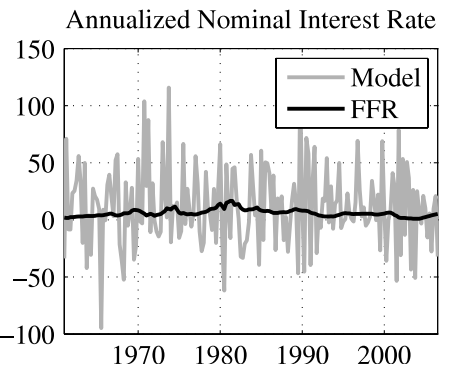
\includegraphics[height=90px]{figs/implied_ffr/nominal_2_collard.png} &
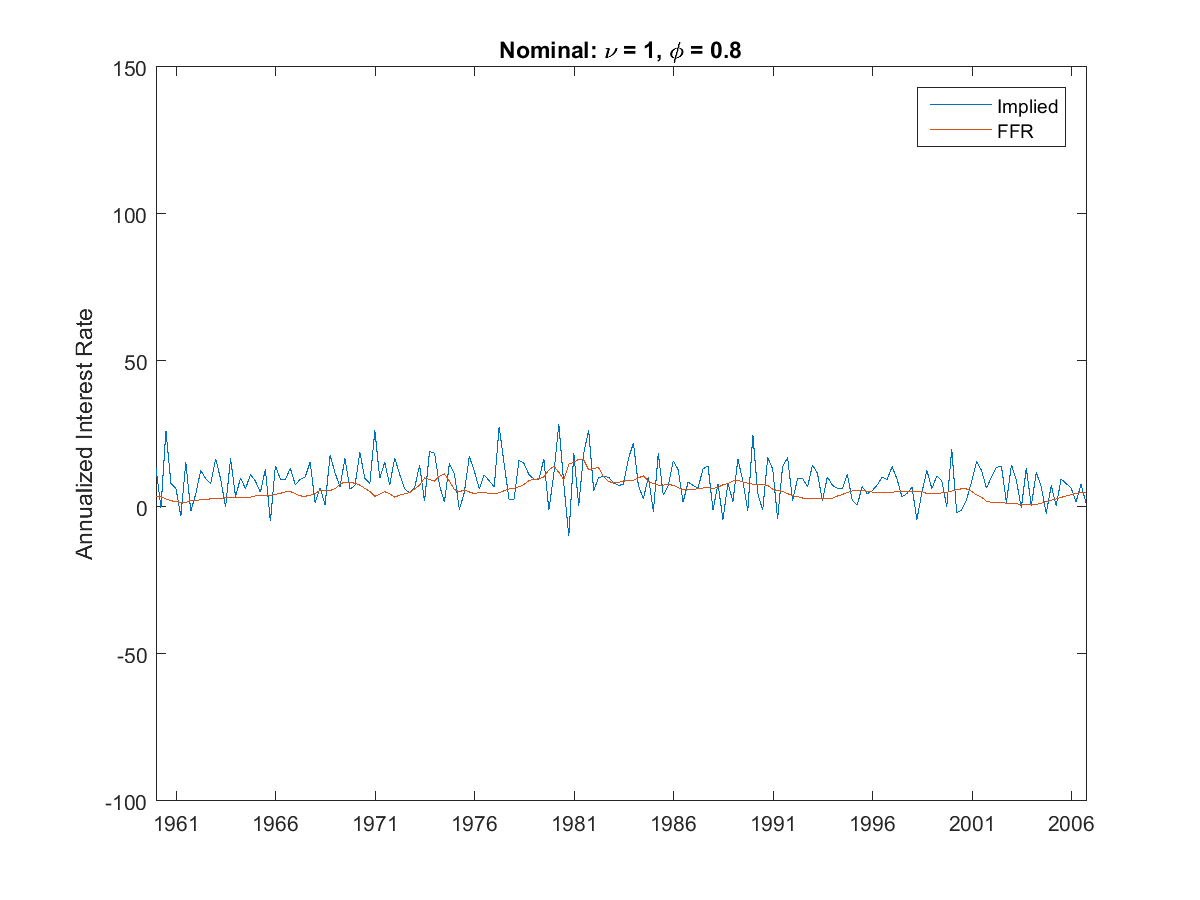
\includegraphics[height=90px]{figs/implied_ffr/nominal_2.png} \\
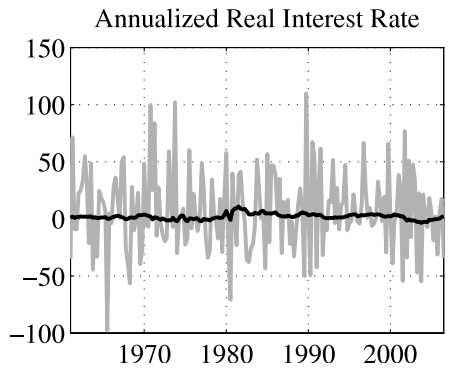
\includegraphics[height=90px]{figs/implied_ffr/real_2_collard.png} &
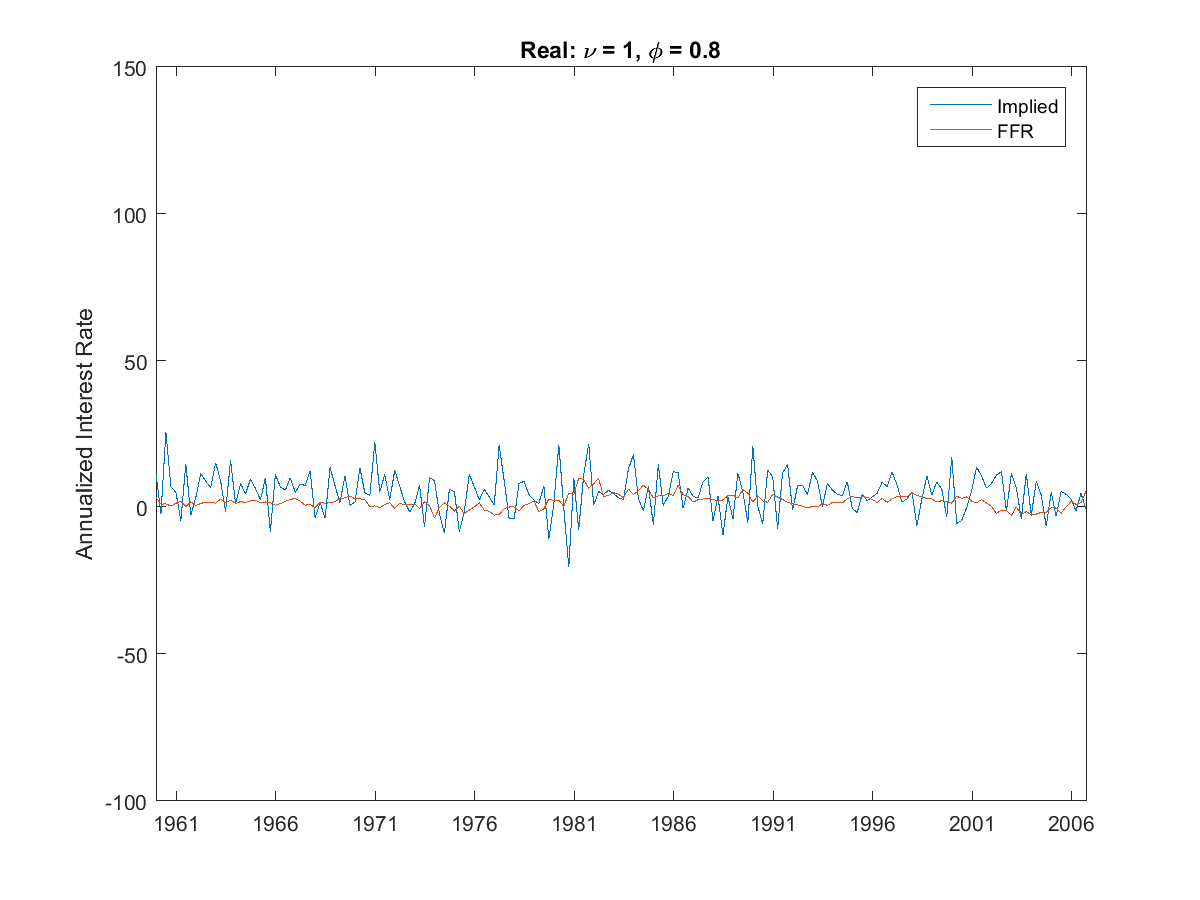
\includegraphics[height=90px]{figs/implied_ffr/real_2.png} \\
\cite{collard11} & Li (2016)
\end{tabular}
\end{center}
\end{frame}

\begin{frame}{Results: NSEP}
\begin{center}
\begin{tabular}{cc}
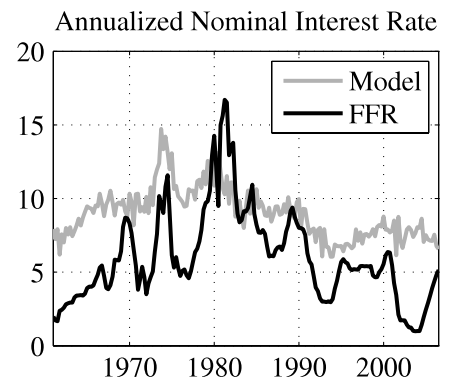
\includegraphics[height=90px]{figs/implied_ffr/nominal_3_collard.png} &
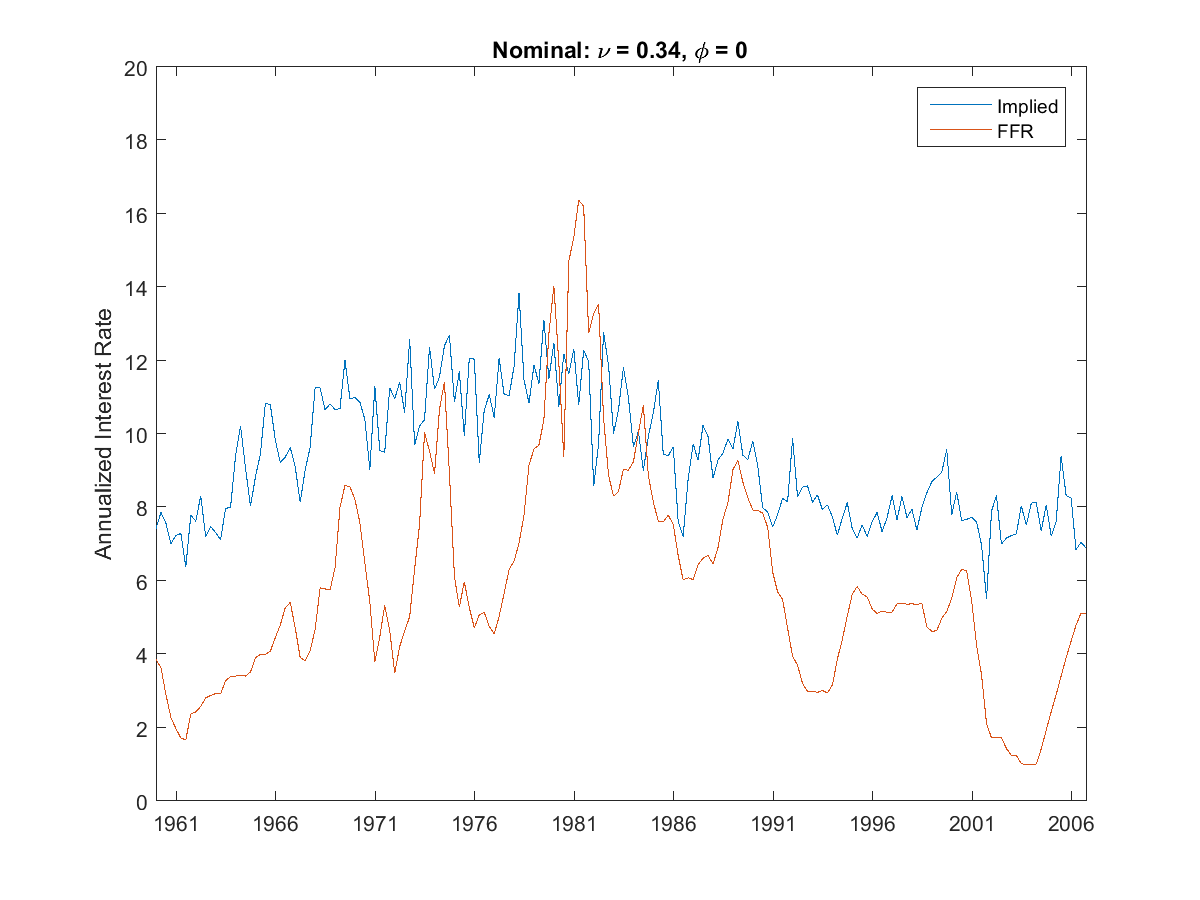
\includegraphics[height=90px]{figs/implied_ffr/nominal_3.png} \\
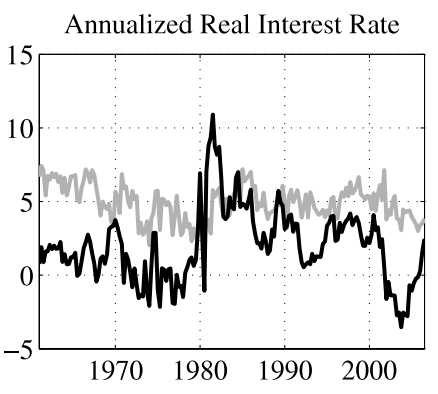
\includegraphics[height=90px]{figs/implied_ffr/real_3_collard.png} &
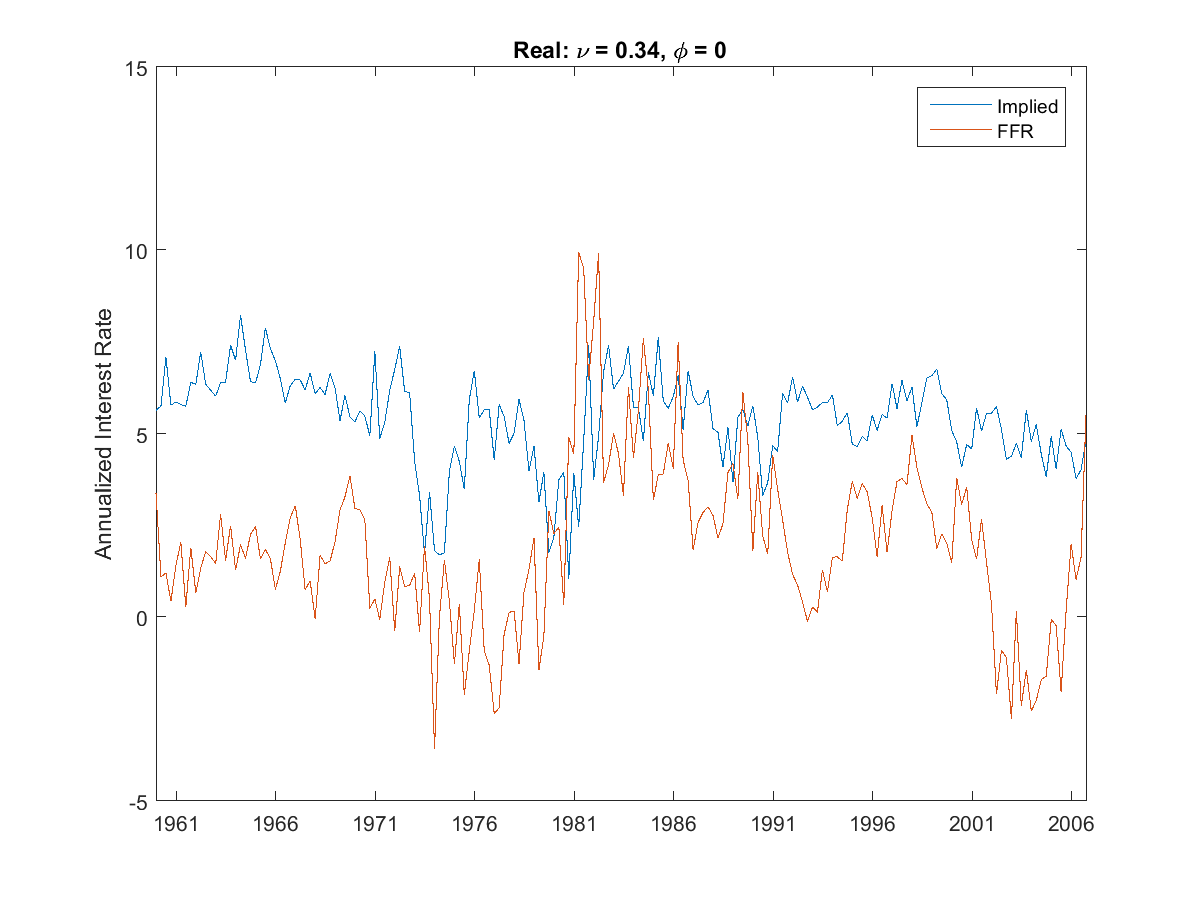
\includegraphics[height=90px]{figs/implied_ffr/real_3.png} \\
\cite{collard11} & Li (2016)
\end{tabular}
\end{center}
\end{frame}

\begin{frame}{Results: NSEP + HP}
\begin{center}
\begin{tabular}{cc}
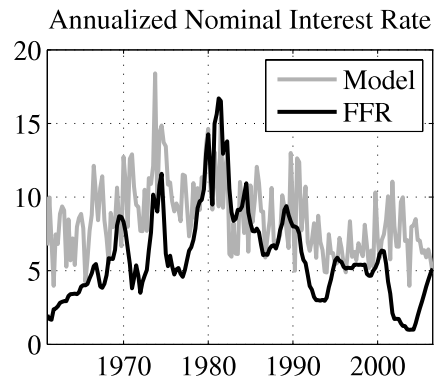
\includegraphics[height=90px]{figs/implied_ffr/nominal_4_collard.png} &
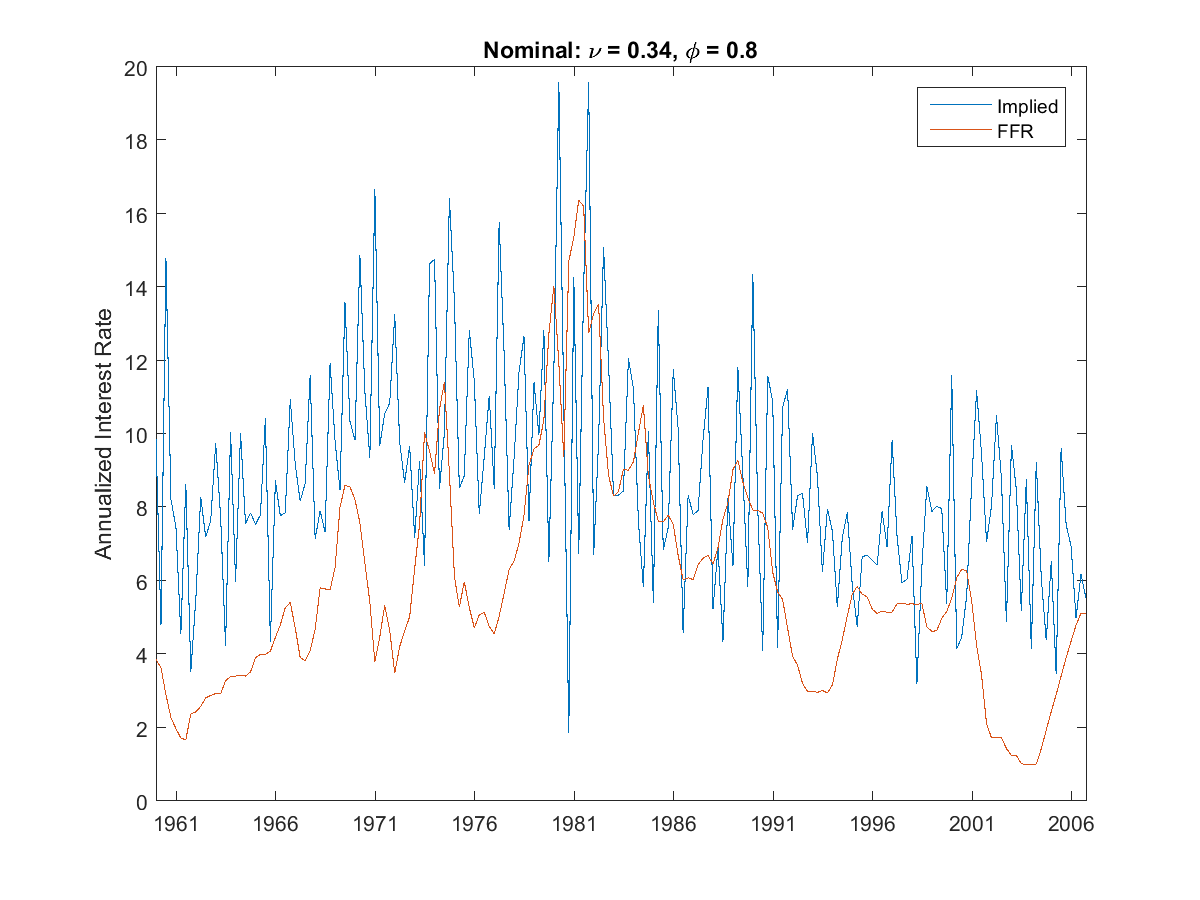
\includegraphics[height=90px]{figs/implied_ffr/nominal_4.png} \\
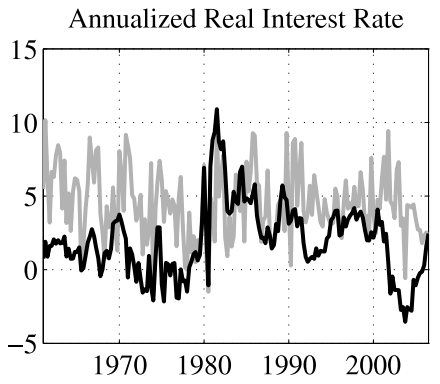
\includegraphics[height=90px]{figs/implied_ffr/real_4_collard.png} &
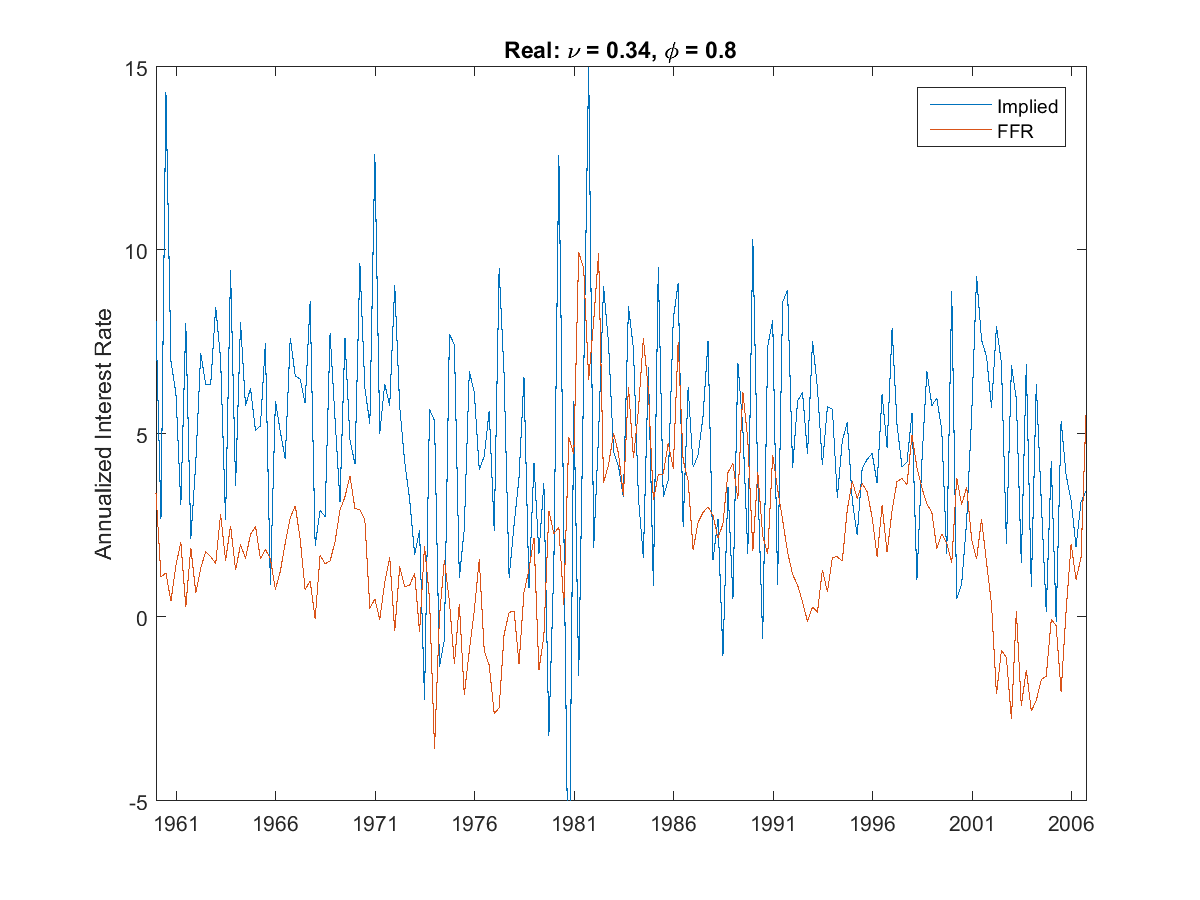
\includegraphics[height=90px]{figs/implied_ffr/real_4.png} \\
\cite{collard11} & Li (2016)
\end{tabular}
\end{center}
\end{frame}

\begin{frame}{Impulse Response}
\begin{itemize}
\item Previously estimated VAR(4)
\end{itemize}
$$y_t = A_0 + A_1 y_{t-1} + \ldots + A_4 y_{t-4} + \epsilon_t$$
$$\epsilon_t \overset{\text{iid}}{\sim} N(0, \Sigma)$$
\begin{align*}
y_t &= \begin{bmatrix} \log(\text{real consumption}_t) \\ \text{inflation}_t \\ \text{leisure}_t \\ \log(\text{real disposable income}_t) \\ \log(\text{income less consumption}_t) \\ \text{effective FFR}_t \\ \log(\text{CCI}_t) \end{bmatrix}
\end{align*}
\end{frame}

\begin{frame}{Impulse Response}
\begin{itemize}
\item Want to observe response of $y_t$ to a $\sigma_{FFR}$ shock to the FFR at $t = 0$ (i.e. $\epsilon_{FFR,0} = \sigma_{FFR}$)
\item No other shocks occur: $\epsilon_{i,0} = 0$ for all other covariates, and $\epsilon_t = 0$ for $t > 0$
\item Compute by iterating forward:
\begin{center}
$\Delta y_0 = \begin{bmatrix} \epsilon_{c,0} \\ \epsilon_{\pi,0} \\ \epsilon_{\ell,0} \\ \epsilon_{RDI,0} \\ \epsilon_{YMC,0} \\ \epsilon_{FFR,0} \\ \epsilon_{CCI,0} \end{bmatrix} = \begin{bmatrix} 0 \\ 0 \\ 0 \\ 0 \\ 0 \\ \sigma_{FFR} \\ 0 \end{bmatrix}$, \quad
\begin{tabular}{l}
$\Delta y_1= A_1 (\Delta y_0)$, \\ \\
$\Delta y_2 = A_1 (\Delta y_1) + A_2 (\Delta y_0)$, \\ \\
$\ldots$
\end{tabular}
\end{center}
where $\Delta y_t = y_t^\text{shock} - y_t^\text{no shock}$
\end{itemize}
\end{frame}

\begin{frame}{Problems}
\end{frame}

\begin{frame}{Next}
\begin{itemize}
\item Get confidence intervals for impulse response via \cite{kilian98}
\item Monte Carlo experiment
\item \textbf{Heterogeneous preferences}
\end{itemize}
\end{frame}

\begin{frame}{References}
\bibliographystyle{../refs/econ}
\bibliography{../refs/refs}
\end{frame}

\end{document}